%!TEX root = ./template-skripsi.tex
%-------------------------------------------------------------------------------
%                            	BAB IV
%               		KESIMPULAN DAN SARAN
%-------------------------------------------------------------------------------

\chapter{HASIL DAN PEMBAHASAN}

\section{\textit{Sprint} 1}

\begin{longtable}{@{}|p{0.5cm}|p{4cm}|p{6cm}|p{2cm}|@{}}
	\caption{\textit{Sprint 1 Backlog}}\\	
	\hline
	\textbf{No} & \textbf{Story} & \textbf{Task} & \textbf{Status} \\
	\hline
	1 & Fitur pencarian pengguna & Menerapkan \textit{mock-up} tampilan halaman hasil pencarian dan pencarian \textit{search engine} & belum \\
	\cline{3-4}
	& & Membuat \textit{mock-up} tampilan halaman hasil pencarian dan pencarian \textit{search engine} & selesai \\
	\cline{3-4}
	& & Membuat \textit{web service} untuk tampilan halaman hasil pencarian dan pencarian \textit{search engine} & belum \\
	\cline{1-4}
	2 & Fitur \textit{staff} & Menerapkan tampilan login, daftar, tambah staff & belum \\
	\cline{3-4}
	& & Membuat \textit{mock-up} tampilan login, daftar, tambah staff & selesai \\
	\cline{3-4}
	& & Membuat \textit{web service} untuk tampilan login, daftar, tambah staff \textit{search engine} & belum \\
	\cline{1-4}  
	3 & Fitur \textit{page ranking} & Menerapkan \textit{mock-up} tampilan status \textit{page ranking} \textit{search engine} & belum \\
	\cline{3-4}
	& & Membuat \textit{mock-up} tampilan status \textit{page ranking} \textit{search engine} & belum \\
	\cline{3-4}
	& & Membuat \textit{web service} untuk tampilan halaman \textit{page ranking} \textit{search engine} & belum \\
	\cline{3-4}
	
	& & Membuat \textit{mock-up} tampilan peta situs \textit{search engine} & selesai \\
	\cline{1-4}
	\hline
	\hline
	& & Menerapkan \textit{mockup} tampilan peta situs & belum \\
	\cline{1-4}
	
\end{longtable}


\begin{enumerate}[label=\alph*)., leftmargin=1\parindent]
	\item{Penentuan Aturan Desain}
	
	Pada \textit{sprint} ini akan dilakukan perancangan tampilan untuk \textit{search engine} ONE (\textit{Omniscience Network Extractor}) dilakukan dengan perangkat lunak Figma dan Adobe Illustrator. Untuk memudahkan proses dalam perancangan tampilan untuk \textit{search engine} yang akan dibangun, diperlukan adanya suatu sistem desain untuk \textit{sizing}, \textit{spacing} dan \textit{color} atau warna.
	
	Dalam sistem desain untuk \textit{spacing} dan \textit{sizing} digunakan seperti tabel berikut
	
	\begin{table}[H]
		\caption{\textit{Sistem desain \textit{sizing} dan \textit{spacing}}}
		\label{Sistem desain sizing dan spacing}
		\includegraphics[keepaspectratio, width=13cm]{gambar/g-109.png}
	\end{table}
	
	Untuk sistem desain warna, warna biru \textit{navy} digunakan sebagai warna utama tampilan \textit{search engine}. Adapun \textit{shades} dari warna utama yaitu \textit{navy} adalah sebagai berikut. Warna \textit{shades} ditentukan dengan cara mengatur nilai \textit{hue}, \textit{saturation} dan \textit{lightning} dari warna utama.
	
	
	\begin{figure}[H]
		\centering
		\includegraphics[keepaspectratio, width=13cm]{gambar/g-110.png}
		\caption{Desain Penelitian}
		\label{gambar:g-110.png}
	\end{figure}
	
	Hal pertama yang dilakukan dalam pembuatan tampilan dari \textit{search engine} adalah mendesain sebuah logo. Sebuah logo digunakan sebagai identitas bagi \textit{search engine} yang akan dibuat tentulah harus mempunyai makna. Logo yang akan dibuat berbentuk "O" melambangkan huruf pertama dari nama search engine tersebut yaitu "ONE". Tanpa warna, logo pola jaring akan terlihat dalam lingkaran berbentuk O yang melambangkan suatu hubungan dari banyaknya sebuah situs. Untuk pewarnaan, digunakan warna oranye yang melambangkan huruf O dari nama \textit{search engine} tersebut, warna \textit{navy} melambangkan huruf N dari nama \textit{search engine} dan warna \textit{eclipse} melambangkan huruf terakhir dari \textit{search engine} tersebut yaitu E.
	
	
	\begin{figure}[H]
		\centering
		\includegraphics[keepaspectratio, width=13cm]{gambar/g-111.png}
		\caption{Desain Logo ONE \textit{Search Engine}}
		\label{gambar:g-111.png}
	\end{figure}
	
	\begin{figure}[H]
		\centering
		\includegraphics[keepaspectratio, width=13cm]{gambar/g-113.png}
		\caption{Desain sistem warna pada logo ONE}
		\label{gambar:g-113.png}
	\end{figure}
	
	Terdapat dua bagian dari tampilan \textit{search engine}, yaitu bagian untuk admin untuk manajemen \textit{search engine} dan tampilan untuk \textit{pengguna}.
	
	Menurut \citep{refactoringui}, jenis font dapat ditentukan dengan observasi jenis \textit{font} yang digunakan dari aplikasi lain yang sudah ada di pasaran. Pada dasarnya, aplikasi yang sudah ada di pasasran memiliki beberapa orang perancang yang memiliki pengalaman lebih mengenai \textit{typography} untuk menentukan jenis \textit{font} yang akan mereka gunakan biasanya dengan telah memperhitungkan berbagai faktor. Setelah melakukan observasi pada aplikasi besar yang ada pada pasaran, peneliti memutuskan untuk menggunakan \textit{font} \textit{Inter} sebagai jenis \textit{font} utama pada aplikasi dikarenakan jenis \textit{font} ini sudah banyak sekali digunakan pada aplikasi besar yang terdapat di pasaran dan bersifat \textit{open source}.
	
	Dalam penentuan \textit{white spacing} dari setiap komponen yang akan dibuat, penulis menggunakan metode \textit{decremental} seperti yang telah dibahas sebelumnya. Pemberian \textit{white spacing} secara \textit{decremental} adalah sebuah cara untuk menemukan nilai \textit{white spacing} yang cocok digunakan pada komponen yang akan dibuat dengan cara memberikan nilai awal \textit{white spacing} yang besar kepada komponen yang akan dibuat dan mengurangi nilai \textit{white spacing}-nya secara bertahap sampai dapat dikatakan cocok. Dalam pemberian \textit{white spacing} penulis menggunakan sistem desain \textit{white spacing} dan \textit{sizing} yang telah ditentukan sebelumnya.
	
	
	\begin{figure}[H]
		\centering
		\includegraphics[keepaspectratio, width=6cm]{gambar/example-whitespace-decremental-1.png}
		\caption{Pemberian nilai \textit{white spacing} awal yang besar terhadap komponen \textit{button}}
		\label{gambar:example-whitespace-decremental-1.png}
	\end{figure}
	
	
	\begin{figure}[H]
		\centering
		\includegraphics[keepaspectratio, width=6cm]{gambar/example-whitespace-decremental-2.png}
		\caption{Pemberian nilai \textit{white spacing} secara \textit{decremental} terhadap komponen \textit{button} sehingga \textit{white spacing} yang diberikan terasa cocok}
		\label{gambar:example-whitespace-decremental-2.png}
	\end{figure}

	\item{Merancang tampilan peta situs}
	\begin{figure}[H]
		\centering
		\includegraphics[keepaspectratio, width=15cm]{gambar/uiux_sitemap.png}
		\caption{Rancangan tampilan peta situs}
		\label{gambar:uiux_sitemap.png}
	\end{figure}


	Pada halaman ini disajikan daftar situs dengan bentuk graf tiga dimensi.
	
	\item{Merancang tampilan \textit{staff}}
	\begin{figure}[H]
		\centering
		\includegraphics[keepaspectratio, width=13cm]{gambar/uiux_staff_login.png}
		\caption{Rancangan tampilan peta login untuk \textit{staff}}
		\label{gambar:uiux_staff_login.png}
	\end{figure}

	Pada halaman ini \textit{staff} dapat melakukan \textit{login} dengan akun mereka untuk masuk ke \textit{dashboard}.
	
	\begin{figure}[H]
		\centering
		\includegraphics[keepaspectratio, width=13cm]{gambar/uiux_staff_add.png}
		\caption{Rancangan tampilan untuk menambahkan \textit{staff}}
		\label{gambar:uiux_staff_add.png}
	\end{figure}

	Pada halaman ini \textit{admin} dapat menambahkan staff baru dengan mengisi formulir yang telah disediakan.

	\begin{figure}[H]
		\centering
		\includegraphics[keepaspectratio, width=10cm]{gambar/uiux_update_profile.png}
		\caption{Rancangan tampilan mengubah profile bagi \textit{staff}}
		\label{gambar:uiux_update_profile.png}
	\end{figure}

	
	Pada halaman ini \textit{staff} dapat mengubah informasi pribadi mereka.
	
	
	\item{Merancang tampilan pencarian}
	
	
	\begin{figure}[H]
		\centering
		\includegraphics[keepaspectratio, width=10cm]{gambar/uiux_search.png}
		\caption{Rancangan tampilan pencarian}
		\label{gambar:uiux_search.png}
	\end{figure}

	Pada halaman ini pengguna dapat melakukan pencarian halaman web yang mereka inginkan dengan memasukan kata kunci yang ingin pengguna cari ke dalam kolom yang telah disediakan lalu tekan tombol \textit{enter}. Setelah itu pengguna akan dialihkan ke halaman hasil pencarian.
	
	
	
	\begin{figure}[H]
		\centering
		\includegraphics[keepaspectratio, width=15cm]{gambar/uiux_search_result.png}
		\caption{Rancangan tampilan hasil pencarian}
		\label{gambar:uiux_search_result.png}
	\end{figure}

	Pada halaman ini pengguna dapat melihat hasil pencarian yang mereka ingingkan. Pada saat pengguna menekan salah satu tautan yang tersedia, pengguna akan dialihkan ke situs dalam \textit{tab} baru. Pengguna juga dapat melihat hasil pencarian mereka dalam bentuk graf tiga dimensi dengan menekan tombol \textit{sitemap}.

\end{enumerate}

%
%\subsection{Halaman \textit{Page Rank Matrix}}
%
%Pada halaman \textit{page rank matrix} admin dapat melihat nilai \textit{page rank matrix} per-domain atau seluruh domain. Pembuatan halaman ini bertujuan agar memudahkan sisi admin dalam melihat \textit{page rank matrix} dari suatu domain ataupun seluruh domain yang berhasil di-\textit{crawl}. Halaman ini tersedia dalam bentuk tiga dimensi dan dua dimensi. Pembuatan halaman ini dalam graf tiga dimensi bertujuan untuk mempermudah pengguna dalam melihat \textit{domain} yang direpresentasikan dengan titik dan garis yang merepresentasikan \textit{outgoing} link dari setiap domain yang ada.
%
%
%\begin{figure}[H]
%	\centering
%	\includegraphics[keepaspectratio, width=13cm]{gambar/page_rank_matrix_visualizer.png}
%	\caption{Desain tampilan \textit{page rank matrix} per-domain atau seluruh domain dalam bentuk dua dimensi}
%	\label{gambar:page_rank_matrix_visualizer.png}
%\end{figure}
%
%\begin{figure}[H]
%	\centering
%	\includegraphics[keepaspectratio, width=13cm]{gambar/pagerank-matrix-3d.png}
%	\caption{Desain tampilan \textit{page rank matrix} per-domain atau seluruh domain dalam bentuk tiga dimensi}
%	\label{gambar:pagerank_matrix_3d.png}
%\end{figure}
%
%
%Adapun routing tabel dari halaman ini adalah sebagai berikut
%
%
%\begin{table}[H]
%	\centering
%	\caption{\textit{Routing Table Halaman Dashboard Admin}}
%	\label{uat}
%	\begin{tabular}{@{} |p{0.5cm}|p{3.5cm}| p{1.5cm}|p{2cm}|p{2cm}|p{2cm} |p{2cm}|p{0.5cm}|@{}}
%		\hline
%		\textbf{No.} & \textbf{\textit{Route}} & \textbf{\textit{Method}} & \textbf{\textit{Description}}  & \textbf{\textit{Body}} & \textbf{\textit{Query}} &  \textbf{\textit{Return}} \\
%		\hline
%		1 & /pagerank-matrix & GET & Menampilkan halaman matrix dari suatu atau seluruh domain dalam bentuk 2 dimensi atau 3 dimensi & - & type, domain & View \\
%		\hline
%	\end{tabular}
%\end{table}
%
%
%\subsection{Halaman Kelola Admin}
%
%Pada halaman kelola admin untuk admin berfokus pada pengelolaan admin pada \textit{search engine} yang telah dibuat. Terdapat beberapa fitur seperti \textit{update} admin, tambah admin, list admin dan pencarian admin. Desain tampilan dibuat seperti daftar berguna untuk memudahkan pengguna dalam menavigasi dari satu admin ke admin yang lainnya.  Halaman ini dibuat tidak memenuhi semua \textit{white spacing} yang tersedia bertujuan agar pengguna lebih mudah dalam menginterpretasikan maksud dan fungsi dari halaman yang sedang dibuka.
%
%\begin{figure}[H]
%	\centering
%	\includegraphics[keepaspectratio, width=13cm]{gambar/managa_admin.png}
%	\caption{Desain tampilan kelola admin \textit{search engine}}
%	\label{gambar:managa_admin.png}
%\end{figure}
%
%Pada tombol tambah admin, admin akan dinavigasikan ke halaman formulir tambah admin.
%
%\begin{figure}[H]
%	\centering
%	\includegraphics[width=16cm]{gambar/add-admin.png}
%	\caption{Desain tampilan update admin \textit{search engine}}
%	\label{gambar:add-admin.png}
%\end{figure}
%
%Untuk tombol update pada halaman kelola admin, admin akan dinavigasikan ke halaman update admin guna mengupdate informasi mengenai admin.
%
%\begin{figure}[H]
%	\centering
%	\includegraphics[keepaspectratio, width=13cm]{gambar/login-admin.png}
%	\caption{Desain tampilan update admin \textit{search engine}}
%	\label{gambar:login-admin.png}
%\end{figure}
%
%
%Adapun routing tabel dari halaman ini adalah sebagai berikut
%
%
%\begin{longtable}{@{} |p{0.5cm}|p{3.5cm}| p{1.5cm}|p{2cm}|p{2cm}|p{2cm} |p{2cm}|p{0.5cm}|@{}}
%	\caption{\textit{Routing Table Halaman Dashboard Admin}}\\
%	\hline
%	\textbf{No.} & \textbf{\textit{Route}} & \textbf{\textit{Method}} & \textbf{\textit{Description}}  & \textbf{\textit{Body}} & \textbf{\textit{Query}} &  \textbf{\textit{Return}} \\
%	\hline
%	1 & /api/v1/admins & GET & Mendapatkan daftar admin \textit{crawler} & -  &  page, limit, roles, query& JSON \\
%	\hline
%	2 & /api/v1/admins/:id /delete & DELETE & Menghapus admin & -  &  -&JSON \\
%	\hline
%	3 & /api/v1/admins/:id /update & PATCH & Mengupdate admin & firstName, lastName, username, role, status, email, profilePictureUrl  &  - &JSON \\
%	\hline
%	4 & /api/v1/admins/:id & GET & Mendapatkan data admin & - &  - & JSON \\
%	\hline
%	5 & /api/v1/admins/:id /create & POST & Menambahkan admin & firstName, lastName, username, role, status, email, profilePictureUrl  &  - &JSON \\
%	\hline
%	6 & /dashboard/admins & GET & Menampilkan halaman kelola & - &  - & View \\
%	\hline
%	7 & /dashboard/admins
%	/add & GET & Menampilkan form tambah admin & - &  - & View \\
%	\hline
%	8 & /dashboard/admins
%	/:id/update & GET & Menampilkan form update admin & - &  - & View \\
%	\hline
%\end{longtable}
%
%
%\subsection{Halaman Peta Situs Admin}
%
%Pada halaman peta situs untuk admin, admin dapat melihat semua situs yang berhasil di-\textit{crawling} dalam bentuk graf 3 dimensi. Graf 3 dimensi dipilih agar visualisasi dari semua link terlihat menarik dan mudah untuk dinavigasi oleh pengguna. Titik dari graf ini adalah sebuah situs dan sisi dari grafnya adalah \textit{outgoing link}. Admin juga dapat mengelola \textit{outgoing link} dari sebuah situs dalam halaman ini. Halaman dibuat dalam tema gelap bertujuan untuk menciptakan suasana luar angkasa dengan titik dari graf melambangkan planet planet yang ada di luar angkasa. Halaman ini dapat diakses dengan menekan tombol "\textit{3D Graph}" pada navigasi \textit{header} yang terdapat di atas halaman web.
%
%\begin{figure}[H]
%	\centering
%	\includegraphics[keepaspectratio, width=13cm]{gambar/admin-sitemap.png}
%	\caption{Desain tampilan peta situs untuk admin \textit{search engine}}
%	\label{gambar:admin-sitemap.png}
%\end{figure}
%
%
%Adapun routing tabel dari halaman ini adalah sebagai berikut
%
%\begin{longtable}{@{} |p{0.5cm}|p{3.5cm}| p{1.5cm}|p{2cm}|p{2cm}|p{2cm} |p{2cm}|p{0.5cm}|@{}}
%	
%	\caption{\textit{Routing Table Halaman Peta Situs Admin}}\\
%	\hline
%	\textbf{No.} & \textbf{\textit{Route}} & \textbf{\textit{Method}} & \textbf{\textit{Description}}  & \textbf{\textit{Body}} & \textbf{\textit{Query}} &  \textbf{\textit{Return}} \\
%	\hline
%	1 & /api/v1/sites/:id
%	/delete & DELETE & Mendelete suatu situs & -  & - & JSON \\
%	\hline
%	2 & /api/v1/sites/:id
%	/update & UPDATE & Mengupdate suatu situs & title, link  & - & JSON \\\hline
%	3 & /api/v1/sites/:id
%	/outgoing & GET & Mendapatkan semua situs outgoing dari suatu situs & -  & limit, page & JSON \\
%	\hline
%	4 & /api/v1/sites/:id & GET & Mendapatkan informasi dari suatu situs & - & - & JSON \\\hline
%	5 & /dashboard/sitemap & GET & Menampilkan halaman peta situs untuk admin & - & site, mode & View \\
%	\hline
%	\hline
%\end{longtable}
%
%
%\subsection{Halaman Login Admin}
%
%Pada halaman login admin, admin dapat login ke dalam \textit{dashboard} admin dengan menggunakan \textit{email} dan password yang telah disediakan. Halaman \textit{login} dibuat menengah agar mata pengguna hanya fokus ke bagian tengah saja dan membuat pengguna lebih mudah menginterpretasikan maksud dan fungsi dari halaman yang sedang dibuka.
%
%\begin{figure}[H]
%	\centering
%	\includegraphics[keepaspectratio, width=13cm]{gambar/admin-login-page.png}
%	\caption{Desain tampilan \textit{login} admin \textit{search engine}}
%	\label{gambar:admin-login-page.png}
%\end{figure}
%
%
%\begin{table}[H]
%	\centering
%	\caption{\textit{Routing Table Halaman Dashboard Admin}}
%	\label{uat}
%	\begin{tabular}{@{} |p{0.5cm}|p{3.5cm}| p{1.5cm}|p{2cm}|p{2cm}|p{2cm} |p{2cm}|p{0.5cm}|@{}}
%		\hline
%		\textbf{No.} & \textbf{\textit{Route}} & \textbf{\textit{Method}} & \textbf{\textit{Description}}  & \textbf{\textit{Body}} & \textbf{\textit{Query}} &  \textbf{\textit{Return}} \\
%		\hline
%		1 & /api/v1/login & GET & Mendapatkan daftar admin \textit{crawler} & email, password  & - & JSON \\ \hline
%		2 & /dashboard/login & POST & Menampilkan halaman login dashboard untuk admin & - & - & View \\
%		\hline
%	\end{tabular}
%\end{table}
%
%\subsection{Halaman Pencarian Pengguna}
%
%Pada halaman pencarian untuk pengguna, pengguna dapat melakukan pencarian pada halaman ini. Terdapat dua menu pada bagian \textit{header} yang dapat pengguna akses yaitu ranking situs dan peta web. Pada halaman ini juga disediakan pencarian pengguna sebelumnya. Bagian \textit{recent searches} betujuan untuk memudahkan pengguna dalam mencari kata pencarian yang pernah dicari sebelumnya. Halaman ini dibuat tidak memenuhi \textit{white spacing} yang tersedia bertujuan agar pengguna lebih mudah dalam menginterpretasikan maksud dan fungsi dari halaman yang sedang dibuka.  Halaman ini dibuat tidak memenuhi semua \textit{white spacing} yang tersedia bertujuan agar pengguna lebih mudah dalam menginterpretasikan maksud dan fungsi dari halaman yang sedang dibuka.
%
%\begin{figure}[H]
%	\centering
%	\includegraphics[keepaspectratio, width=13cm]{gambar/user-search-page.png}
%	\caption{Desain tampilan halaman pencarian untuk pengguna}
%	\label{gambar:user-search-page.png}
%\end{figure}
%
%
%\begin{table}[H]
%	\centering
%	\caption{\textit{Routing Table Halaman Pencarian Pengguna}}
%	\label{uat}
%	\begin{tabular}{@{} |p{0.5cm}|p{3.5cm}| p{1.5cm}|p{2cm}|p{2cm}|p{2cm} |p{2cm}|p{0.5cm}|@{}}
%		\hline
%		\textbf{No.} & \textbf{\textit{Route}} & \textbf{\textit{Method}} & \textbf{\textit{Description}}  & \textbf{\textit{Body}} & \textbf{\textit{Query}} &  \textbf{\textit{Return}} \\
%		\hline
%		1 & /api/v1/search & GET & Mendapatkan daftar admin \textit{crawler} & - & - & query \\ \hline
%		2 & / & GET & Menapilkan halaman pencarian untuk pengguna & - & - & View \\
%		\hline
%	\end{tabular}
%\end{table}
%
%\subsection{Halaman Peta Situs Pengguna}
%
%Sama seperti peta situs untuk admin, pengguna dapat melihat semua situs yang berhasil di-\textit{crawling} dalam bentuk graf 3 dimensi. Graf 3 dimensi dipilih agar visualisasi dari semua link terlihat menarik dan mudah untuk dinavigasi oleh pengguna. Titik dari graf ini adalah sebuah situs dan sisi dari grafnya adalah \textit{outgoing link}. Pengguna dapat melihat \textit{outgoing link} dari sebuah situs yang difokuskan pada bagian kanan layar. Pengguna juga dapat memfokuskan \textit{link} yang lain dengan menekan salah satu dari titik titik yang ada. Halaman dibuat dalam tema gelap bertujuan untuk menciptakan suasana luar angkasa dengan titik dari graf melambangkan planet planet yang ada di luar angkasa.
%
%\begin{figure}[H]
%	\centering
%	\includegraphics[keepaspectratio, width=13cm]{gambar/user-sitemap.png}
%	\caption{Desain tampilan peta situs untuk pengguna \textit{search engine}}
%	\label{gambar:user-sitemap.png}
%\end{figure}
%
%
%Adapun routing tabel dari halaman ini adalah sebagai berikut
%
%\begin{table}[H]
%	\centering
%	\caption{\textit{Routing Table Halaman Peta Situs Pengguna}}
%	\label{uat}
%	\begin{tabular}{@{} |p{0.5cm}|p{3.5cm}| p{1.5cm}|p{2cm}|p{2cm}|p{2cm} |p{2cm}|p{0.5cm}|@{}}
%		\hline
%		\textbf{No.} & \textbf{\textit{Route}} & \textbf{\textit{Method}} & \textbf{\textit{Description}}  & \textbf{\textit{Body}} & \textbf{\textit{Query}} &  \textbf{\textit{Return}} \\
%		\hline
%		1 & /api/v1/sites/:id
%		/outgoing & GET & Mendapatkan semua situs outgoing dari suatu situs & -  & limit, page & JSON \\
%		\hline
%		2 & /api/v1/sites/:id & GET & Mendapatkan informasi dari suatu situs & - & - & JSON \\\hline
%		3 & /sitemap & GET & Menampilkan halaman peta situs untuk pengguna  & - & site, mode & View \\
%		\hline
%	\end{tabular}
%\end{table}
%
%\subsection{Halaman Hasil Pencarian Pengguna}
%
%Halaman ini merupakan halaman setelah pengguna mamasukan kata pencarian pada \textit{search engine}. Pada halaman ini menyajikan situs-situs yang relevan berdasarkan kata pencarian yang pengguna berikan. Pengguna juga dapat menambahkan parameter tambahan seperti \textit{sort by} dan sebuah \textit{filter} untuk membuat hasil pencarian lebih akurat untuk pengguna. Hasil pencarian dibuat tidak mengisi seluruh \textit{white space} agar pengguna lebih mudah menavigasi hasil pencarian dengan mengurangi pergerakan mata pengguna. Pada hasil pencarian juga disediakan tombol tanda panah miring bertujuan untuk mengantarkan pengguna ke halaman peta situs dan melihat situs hasil pencarian tersebut dalam  bentuk tiga dimensi. Halaman ini dibuat tidak memenuhi semua \textit{white spacing} yang tersedia bertujuan agar pengguna lebih mudah dalam menginterpretasikan maksud dan fungsi dari halaman yang sedang dibuka.
%
%\begin{figure}[H]
%	\centering
%	\includegraphics[keepaspectratio, width=10cm]{gambar/user-search-result.png}
%	\caption{esain tampilan halaman hasil pencarian}
%	\label{gambar:user-search-result.png}
%\end{figure}
%
%
%Adapun routing tabel dari halaman ini adalah sebagai berikut
%
%\begin{longtable}{@{} |p{0.5cm}|p{3.5cm}| p{1.5cm}|p{2cm}|p{2cm}|p{2cm} |p{2cm}|p{0.5cm}|@{}}
%	
%	\caption{\textit{Routing Table Halaman Hasil Pencarian Pengguna}}\\
%	\hline
%	\textbf{No.} & \textbf{\textit{Route}} & \textbf{\textit{Method}} & \textbf{\textit{Description}}  & \textbf{\textit{Body}} & \textbf{\textit{Query}} &  \textbf{\textit{Return}} \\
%	\hline
%	1 & /api/v1/search
%	/outgoing & GET & Mendapatkan semua situs yang terkait dengan kata kunci yang diberikan & -  & limit, page, query, filters, sort & JSON \\
%	\hline
%	2 & /search & GET & Menampilkan halaman hasil pencarian berdasarkan kata kunci yang diberikan & - & limit, page, query, filters, sort & View \\\hline
%\end{longtable}
%
%
%\subsection{Halaman Ranking Situs}
%
%Pada halaman ini akan menampilkan ranking dari semua url yang berhasil di-\textit{crawl}. Halaman perankingan situs dibuat tidak mengisi seluruh \textit{white space} agar pengguna lebih mudah menavigasi ranking situs dengan mengurangi pergerakan mata pengguna. Pada ranking juga disediakan tombol tanda panah miring bertujuan untuk mengantarkan pengguna ke halaman peta situs dan melihat situs hasil pencarian tersebut dalam  bentuk tiga dimensi. Halaman ini dibuat tidak memenuhi \textit{white spacing} yang tersedia bertujuan agar pengguna lebih mudah dalam menginterpretasikan maksud dan fungsi dari halaman yang sedang dibuka.
%
%\begin{figure}[H]
%	\centering
%	\includegraphics[keepaspectratio, width=13cm]{gambar/user-page-ranking-page.png}
%	\caption{Desain tampilan ranking halaman}
%	\label{gambar:user-page-ranking-page.png}
%\end{figure}
%
%
%
%Adapun routing tabel dari halaman ini adalah sebagai berikut
%
%\begin{table}[H]
%	\centering
%	\caption{\textit{Routing Table Halaman Peta Situs Pengguna}}
%	\label{uat}
%	\begin{tabular}{@{} |p{0.5cm}|p{3.5cm}| p{1.5cm}|p{2cm}|p{2cm}|p{2cm} |p{2cm}|p{0.5cm}|@{}}
%		\hline
%		\textbf{No.} & \textbf{\textit{Route}} & \textbf{\textit{Method}} & \textbf{\textit{Description}}  & \textbf{\textit{Body}} & \textbf{\textit{Query}} &  \textbf{\textit{Return}} \\
%		\hline
%		1 & /api/v1/ranking
%		/outgoing & GET & Mendapatkan ranking dari semua situs  & -  & limit, page & JSON \\
%		\hline
%		2 & /ranking  & GET & Menampilkan halaman ranking situs & - & limit, page, query, filters, sort & View \\\hline
%	\end{tabular}
%\end{table}

\section{\textit{Sprint} 2}

\begin{longtable}{@{}|p{0.5cm}|p{4cm}|p{6cm}|p{2cm}|@{}}
	\caption{\textit{Sprint 2 Backlog}}\\	
	\hline
	\textbf{No} & \textbf{Story} & \textbf{Task} & \textbf{Status} \\
	\hline
	1 & Fitur pencarian pengguna & Menerapkan \textit{mock-up} tampilan halaman hasil pencarian dan pencarian \textit{search engine} & selesai \\
	\cline{3-4}
	& & Membuat \textit{mock-up} tampilan halaman hasil pencarian dan pencarian \textit{search engine} & selesai (sprint 1) \\
	\cline{3-4}
	& & Membuat \textit{Rest API} untuk tampilan halaman hasil pencarian dan pencarian \textit{search engine} & belum \\
	\cline{1-4}
%	2 & Fitur \textit{page ranking} & Menerapkan \textit{mock-up} tampilan status \textit{page ranking} \textit{search engine} & belum \\
%	\cline{3-4}
%	& & Membuat \textit{mock-up} tampilan status \textit{page ranking} \textit{search engine} & selesai \\
%	\cline{3-4}
%	& & Mengintegrasikan \textit{web service} dengan tampilan halaman \textit{page ranking} \textit{search engine} & belum \\
%	\hline
	2 & Struktur Projek & Merancang struktur projek yang akan digunakan & belum \\
	\cline{1-4}
	
\end{longtable}


\begin{enumerate}[label=\alph*)., leftmargin=1\parindent]
	\item{Penerapan Tampilan Pencarian Pengguna}
	
	Pada tahap ini, dilakukan pengimplementasian \textit{mock-up} tampilan yang telah dibuat pada sprint sebelumnya dengan menggunakan bahasa pemgrograman \textit{Javascript} dengan bantuan pustaka \textit{Vue}.
	
	\begin{figure}[H]
		\centering
		\includegraphics[keepaspectratio, width=13cm]{gambar/view_search_engine_home.png}
		\caption{Tampilan halaman pencarian \textit{search engine}}
		\label{gambar:view_search_engine_home.png}
	\end{figure}
	
	
	\begin{figure}[H]
		\centering
		\includegraphics[keepaspectratio, width=13cm]{gambar/view_search_engine_result.png}
		\caption{Tampilan halaman hasil pencarian \textit{search engine}}
		\label{gambar:view_search_engine_result.png}
	\end{figure}
	
	\item{Perancangan Struktur Kode Projek}
	
	
	Rancangan ini terdiri dari beberapa direktori utama yaitu \textit{api}, \textit{components}, \textit{router} dan \textit{views}. Direktori \textit{api} berfungsi untuk menyimpan segala panggilan \textit{web api} yang dilakukan oleh aplikasi. Direktori \textit{components} berisi komponen-komponen tampilan aplikasi. Direktori \textit{router} berisi dengan pemetaan tampilan aplikasi dan \textit{views} merupakan direktori yang berfungsi sebagai penyimpanan berbagai tampilan layar aplikasi.
	
	\begin{figure}[H]
		\centering
		\includegraphics[keepaspectratio, width=16cm]{gambar/structure-project.png}
		\caption{Tampilan struktur kode projek \textit{search engine}}
		\label{gambar:structure-project.png}
	\end{figure}
%	\item{\textit{Unit Testing}}
%	
%	\begin{longtable}{@{}|p{8cm}|p{3cm}|p{3cm}|@{}}
%		\caption{\textit{Unit Testing} Tampilan Pencarian}\\
%		\hline
%		\textbf{Skenario Pengujian} & \textbf{Sesuai} & \textbf{Tidak Sesuai} \\
%		\hline
%		 Pengguna dapat melakukan pencarian halaman web dengan memasukan kata kunci ke dalam \textit{text input} yang tersedia & \checkmark &  \\
%		\hline
%		Pengguna dapat melihat hasil pencarian setelah melakukan pencarian & \checkmark &  \\
%		\hline
%		Pengguna dapat melihat hasil pencarian lebih banyak menggunakan \textit{pagination} yang terletak pada bawah halaman pencarian & \checkmark &  \\
%		\hline
%	\end{longtable}
%	\item{Perencanaan Sprint 3} 
%	
%%	Pada akhir sprint ini telah dilakukan \textit{review} mengenai fitur yang telah dibuat dengan \textit{stakeholder}. Tidak ditemukan adanya kendala. Perencanaan \textit{Sprint 3} akan dilakukan pengimplementasian desain halaman \textit{crawling}.
%	Pada akhir sprint diadakan perencanaan untuk \textit{sprint 3}. Pada \textit{sprint 3} akan dilakukan desain dan pengimplementasian desain halaman fitur \textit{crawling}.
\end{enumerate}


\section{\textit{Sprint} 3}

\begin{longtable}{@{}|p{0.5cm}|p{4cm}|p{6cm}|p{2cm}|@{}}
	\caption{\textit{Sprint 3 Backlog}}\\	
	\hline
	\textbf{No} & \textbf{Story} & \textbf{Task} & \textbf{Status} \\
	\hline
	1 & Fitur crawling & Menerapkan \textit{mock-up} tampilan status crawling \textit{search engine} & selesai \\
	\cline{3-4}
	& & Membuat \textit{mock-up} tampilan status crawling \textit{search engine} & selesai \\
	\cline{3-4}
	& & Membuat \textit{web service} untuk tampilan halaman status crawling \textit{search engine} & belum \\
	\cline{3-4}
	
\end{longtable}



\begin{enumerate}[label=\alph*)., leftmargin=1\parindent]
	\item{Desain Tampilan Halaman Fitur Crawling}
	\begin{figure}[H]
		\centering
		\includegraphics[keepaspectratio, width=13cm]{gambar/uiux_crawling_overview.png}
		\caption{Tampilan halaman \textit{overview crawling} \textit{search engine}}
		\label{gambar:uiux_crawling_overview.png}
	\end{figure}

	Halaman ini menampilkan ringkasan mengenai fitur \textit{crawling}, pada halaman ini dapat menjalankan tugas \textit{crawling} dengan menekan tombol \textit{start}. Halaman ini juga menyajikan informasi berupa jumlah penggunaan \textit{storage}, jumlah halaman \textit{web} dan jumlah \textit{domains}.

	\begin{figure}[H]
		\centering
		\includegraphics[keepaspectratio, width=13cm]{gambar/uiux_crawling_domains.png}
		\caption{Tampilan halaman \textit{domains crawling} \textit{search engine}}
		\label{gambar:uiux_crawling_domains.png}
	\end{figure}

	Halaman ini menyajikan daftar \textit{domain} yang berhasil ter-\textit{crawl}. Pada setiap domain terdapat informasi dari negara mana \textit{domain} itu berasal dan jumlah halaman web yang ada dalam cakupan \textit{domain} tersebut.


	\begin{figure}[H]
		\centering
		\includegraphics[keepaspectratio, width=13cm]{gambar/uiux_crawling_webpages.png}
		\caption{Tampilan halaman hasil \textit{crawling} halaman \textit{web} \textit{search engine}}
		\label{gambar:uiux_crawling_webpages.png}
	\end{figure}


	Halaman ini menyajikan daftar halaman \textit{web} yang berhasil ter-\textit{crawl}. Pada setiap halaman \textit{web} terdapat informasi dari negara mana halaman \textit{web} itu berasal, URL halaman web tersebut dan skor \textit{pagerank}.

	
	\begin{figure}[H]
		\centering
		\includegraphics[keepaspectratio, width=13cm]{gambar/uiux_crawling_cloudword_webpages.png}
		\caption{Tampilan halaman detail halaman \textit{web} \textit{search engine}}
		\label{gambar:uiux_crawling_cloudword_webpages.png}
	\end{figure}
	
	\item{Penerapan Tampilan Halaman Fitur Crawling}
	
	Pada tahap ini, dilakukan pengimplementasian \textit{mock-up} tampilan yang telah dibuat dengan menggunakan bahasa pemgrograman \textit{Javascript} dengan bantuan pustaka \textit{Vue}.
	
	\begin{figure}[H]
		\centering
		\includegraphics[keepaspectratio, width=13cm]{gambar/view_dashboard_services_crawling_overview.png}
		\caption{Tampilan halaman status \textit{crawling} \textit{search engine}}
		\label{gambar:view_dashboard_services_crawling_overview.png}
	\end{figure}
	
	
	\begin{figure}[H]
		\centering
		\includegraphics[keepaspectratio, width=13cm]{gambar/view_crawling_domain_list.png}
		\caption{Tampilan halaman daftar domain \textit{crawling} \textit{search engine}}
		\label{gambar:view_crawling_domain_list.png}
	\end{figure}		
%
%\item{\textit{Unit Testing}}
%
%\begin{longtable}{@{}|p{5cm}|p{3cm}|p{3cm}|@{}}
%	\caption{\textit{Unit Testing} Tampilan Crawling}\\
%	\hline
%	\textbf{Skenario Pengujian} & \textbf{Sesuai} & \textbf{Tidak Sesuai} \\
%	\hline
%	Pengguna dapat memulai proses \textit{crawling} dengan mengklik tulisan \textit{start} & \checkmark &  \\
%	\hline
%	Pengguna dapat menghentikan jalannya \textit{crawling} dengan mengklik tulisan \textit{stop} & \checkmark &  \\
%	\hline
%	Saat \textit{tab} \textit{domains} diklik, pengguna akan dialihkan ke sub halaman daftar domain & \checkmark &  \\
%	\hline
%	Saat \textit{tab} \textit{webpages} diklik, pengguna akan dialihkan ke sub halaman daftar webpage & \checkmark &  \\
%	\hline
%\end{longtable}

	\item{Pengujian Sprint 3 dan Perencanaan Sprint 4} 
	
	Pada akhir sprint ini telah dilakukan \textit{pengujian} mengenai fitur yang telah dibuat dengan \textit{stakeholder}. Tidak ditemukan adanya kendala. Pada perencanaan \textit{Sprint 4} akan dilakukan pengimplementasian desain \textit{page ranking}.
\end{enumerate}





\section{\textit{Sprint} 4}

\begin{longtable}{@{}|p{0.5cm}|p{4cm}|p{6cm}|p{2cm}|@{}}
	\caption{\textit{Sprint 4 Backlog}}\\	
	\hline
	\textbf{No} & \textbf{Story} & \textbf{Task} & \textbf{Status} \\
	\hline
	1 & Fitur \textit{page ranking} & Menerapkan \textit{mock-up} tampilan status \textit{page ranking} \textit{search engine} & belum \\
	\cline{3-4}
	& & Membuat \textit{mock-up} tampilan status \textit{page ranking} \textit{search engine} & belum \\
	\cline{3-4}
	& & Membuat \textit{web service} untuk tampilan halaman \textit{page ranking} \textit{search engine} & belum \\
	\cline{3-4}
	
	& & Membuat \textit{mock-up} tampilan peta situs \textit{search engine} & selesai (sprint 1) \\
	\cline{3-4}
	& & Menerapkan \textit{mockup} tampilan peta situs & selesai \\
	\cline{1-4}
	
\end{longtable}


\begin{enumerate}[label=\alph*)., leftmargin=1\parindent]
	\item{Penerapan Tampilan Peta Situs}
	
	\begin{figure}[H]
		\centering
		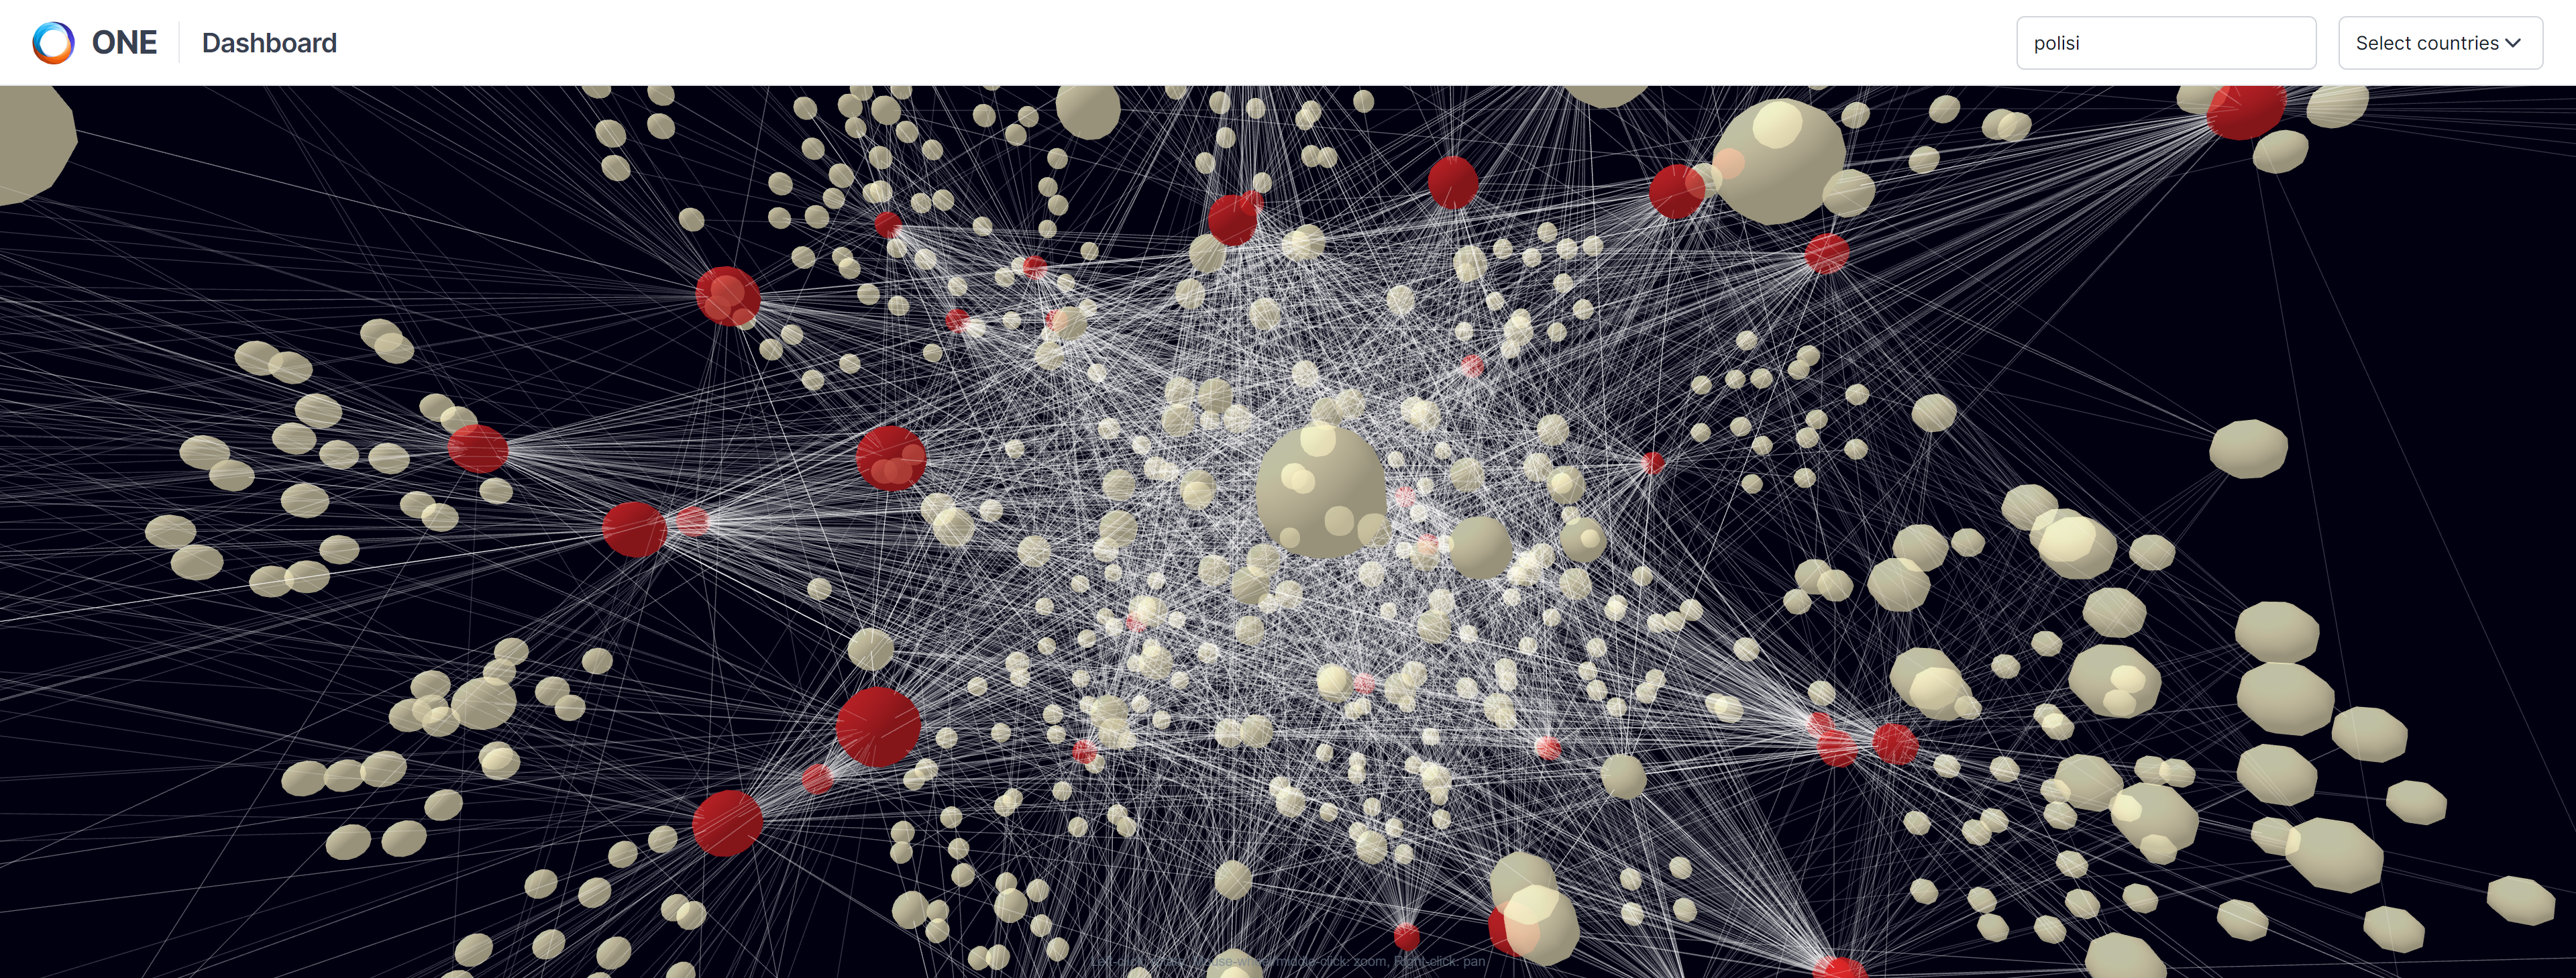
\includegraphics[keepaspectratio, width=13cm]{gambar/view_sitemap.png}
		\caption{Tampilan halaman peta situs}
		\label{gambar:view_sitemap.png}
	\end{figure}		
%
%
%
%	\item{\textit{Unit Testing}}
%
%	\begin{longtable}{@{}|p{5cm}|p{3cm}|p{3cm}|@{}}
%		\caption{\textit{Unit Testing} Tampilan Page Ranking}\\
%		\hline
%		\textbf{Skenario Pengujian} & \textbf{Sesuai} & \textbf{Tidak Sesuai} \\
%		\hline
%		Pengguna dapat mem-\textit{filter} peta situs berdasarkan kata kunci dan negara asal situs & \checkmark &  \\
%
%		\hline
%	\end{longtable}

	\item{Pengujian Sprint 4 dan Perencanaan Sprint 5} 
	
	Pada akhir sprint ini telah dilakukan \textit{pengujian} mengenai fitur yang telah dibuat dengan \textit{stakeholder}. Ditemukan kendala pada penerapan peta situs dimana peta situs untuk semua yang dibuat terasa berat dari sisi performa, sehingga peta situs disederhanakan menjadi hanya menampilkan peta situs setelah pengguna memasukan kata kunci pencarian. Pada perencanaan \textit{Sprint 5} akan dilakukan pembuatan lalu pengimplementasian desain \textit{page ranking} dan pembuatan lalu pengimplementasian desain \textit{document ranking}.
\end{enumerate}

%
%\begin{longtable}{@{}|p{0.5cm}|p{4cm}|p{6cm}|p{2cm}|@{}}
%	\caption{\textit{Sprint 4 Backlog}}\\	
%	\hline
%	\textbf{No} & \textbf{Story} & \textbf{Task} & \textbf{Status} \\
%	\hline
%	1 & Fitur \textit{document ranking} & Menerapkan \textit{mock-up} tampilan status \textit{document ranking} \textit{search engine} & selesai \\
%	\cline{3-4}
%	& & Membuat \textit{mock-up} tampilan status \textit{document ranking} \textit{search engine} & selesai \\
%	\cline{3-4}
%	& & Mengintegrasikan \textit{web service} dengan tampilan halaman\textit{document ranking} \textit{search engine} & belum \\
%	\cline{3-4}
%	\hline
%	
%\end{longtable}
%
%
%\begin{figure}[H]
%	\centering
%	\includegraphics[keepaspectratio, width=13cm]{gambar/view_document_ranking_overview.png}
%	\caption{Tampilan halaman \textit{overview document ranking} \textit{search engine}}
%	\label{gambar:view_document_ranking_overview.png}
%\end{figure}
%
%
%\begin{figure}[H]
%	\centering
%	\includegraphics[keepaspectratio, width=13cm]{gambar/view_document_ranking_search_logs.png}
%	\caption{Tampilan halaman \textit{search logs document ranking} \textit{search engine}}
%	\label{gambar:view_document_ranking_search_logs.png}
%\end{figure}
%
%
%\begin{figure}[H]
%	\centering
%	\includegraphics[keepaspectratio, width=13cm]{gambar/view_document_ranking_words.png}
%	\caption{Tampilan halaman \textit{word list document ranking} \textit{search engine}}
%	\label{gambar:view_document_ranking_words.png}
%\end{figure}
%



\section{\textit{Sprint} 5}


\begin{longtable}{@{}|p{0.5cm}|p{4cm}|p{6cm}|p{2cm}|@{}}
	\caption{\textit{Sprint 5 Backlog}}\\	
	\hline
	\textbf{No} & \textbf{Story} & \textbf{Task} & \textbf{Status} \\
	\hline
	1 & Fitur \textit{page ranking} & Menerapkan \textit{mock-up} tampilan status \textit{page ranking} \textit{search engine} & selesai \\
	\cline{3-4}
	& & Membuat \textit{mock-up} tampilan peta situs \textit{search engine} & selesai (sprint 4) \\
	\cline{3-4}
	& & Membuat \textit{mock-up} tampilan status \textit{page ranking} \textit{search engine} & selesai \\
	\cline{3-4}
	& & Membuat \textit{web service} untuk tampilan halaman \textit{page ranking} \textit{search engine} & belum \\
	\cline{1-4}
	2 & Fitur \textit{staff} & Menerapkan tampilan login, daftar, tambah staff & selesai \\
	\cline{3-4}
	& & Membuat \textit{mock-up} tampilan login, daftar, tambah staff & selesai (sprint 1) \\
	\cline{3-4}
	& & Membuat \textit{web service} untuk tampilan login, daftar, tambah staff \textit{search engine} & belum \\
	\cline{1-4}	
	3 & Fitur \textit{document ranking} & Menerapkan \textit{mock-up} tampilan status \textit{document ranking} \textit{search engine} & selesai \\
	\cline{3-4}
	& & Membuat \textit{mock-up} tampilan status \textit{document ranking} \textit{search engine} & selesai \\
	\cline{3-4}
	& & Membuat \textit{web service} untuk tampilan halaman\textit{document ranking} \textit{search engine} & belum \\
	\cline{3-4}
	\hline
	
\end{longtable}




\begin{enumerate}[label=\alph*)., leftmargin=1\parindent]
	
	\item{Pembuatan \textit{mockup} tampilan \textit{page ranking}}
	
	
	\begin{figure}[H]
		\centering
		\includegraphics[keepaspectratio, width=13cm]{gambar/uiux_pageranking_overview.png}
		\caption{Tampilan halaman \textit{overview page ranking} \textit{search engine}}
		\label{gambar:uiux_pageranking_overview.png}
	\end{figure}


	Halaman ini menampilkan ringkasan mengenai fitur \textit{page ranking}, pada halaman ini dapat menjalankan tugas \textit{page ranking} dengan menekan tombol \textit{start}. Halaman ini juga menyajikan informasi berupa jumlah penggunaan \textit{storage}, jumlah konektivitas antara halaman \textit{web}, jumlah halaman \textit{web}, jumlah halaman \textit{web} yang ada dalam \textit{database}, \textit{wordcloud} dan kata kunci yang paling banyak dicari.
	
	\item{Pembuatan \textit{mockup} tampilan \textit{document ranking}}
	
	\begin{figure}[H]
		\centering
		\includegraphics[keepaspectratio, width=13cm]{gambar/uiux_documentranking_overview.png}
		\caption{Tampilan halaman \textit{overview document ranking} \textit{search engine}}
		\label{gambar:uiux_documentranking_overview.png}
	\end{figure}

	Halaman ini menampilkan ringkasan mengenai fitur \textit{document ranking}, pada halaman ini dapat menjalankan tugas \textit{document ranking} dengan menekan tombol \textit{start}. Halaman ini juga menyajikan informasi berupa kata kata unik, jumlah halaman \textit{web} yang ada dalam \textit{database}, \textit{wordcloud} dan kata kunci yang paling banyak dicari.


	\begin{figure}[H]
		\centering
		\includegraphics[keepaspectratio, width=13cm]{gambar/uiux_documentranking_search_logs.png}
		\caption{Tampilan halaman \textit{overview document ranking} \textit{search logs}}
		\label{gambar:uiux_documentranking_search_logs.png}
	\end{figure}

	Pada halaman \textit{search logs} terdapat daftar kata kata yang pernah pengguna cari dengan \textit{search engine}. Data yang dikumpulkan berupa halaman \textit{web}, kata kunci, \textit{browser} yang pengguna gunakan dan tanggal.

	\begin{figure}[H]
		\centering
		\includegraphics[keepaspectratio, width=13cm]{gambar/uiux_documentranking_words.png}
		\caption{Tampilan halaman daftar kata \textit{document ranking}}
		\label{gambar:uiux_documentranking_words.png}
	\end{figure}

	Halaman ini menyajikan daftar kata kata yang terdapat dalam \textit{database} diurutkan mulai dari jumlah penggunaan. Pada saat pengguna menekan salah satu kata maka pengguna akan diantarkan ke halaman detail kata.


	\begin{figure}[H]
		\centering
		\includegraphics[keepaspectratio, width=10cm]{gambar/uiux_documentranking_word_details.png}
		\caption{Tampilan halaman detail kata \textit{document ranking}}
		\label{gambar:uiux_documentranking_word_details.png}
	\end{figure}

	Pada halaman detail kata, disajikan sebuah daftar halaman \textit{web} yang mengandung kata tersebut.
	
	\item{Penerapan tampilan \textit{page ranking search engine}}
	
	
	\begin{figure}[H]
		\centering
		\includegraphics[keepaspectratio, width=15cm]{gambar/view_page_ranking_overview.png}
		\caption{Tampilan halaman \textit{overview page ranking} \textit{search engine}}
		\label{gambar:view_page_ranking_overview.png}
	\end{figure}

	\item{Penerapan tampilan \textit{staff}}
	
	
	\begin{figure}[H]
		\centering
		\includegraphics[keepaspectratio, width=13cm]{gambar/view_staff_add.png}
		\caption{Tampilan halaman tambah \textit{staff}}
		\label{gambar:view_staff_add.png}
	\end{figure}
	
	
	
	\begin{figure}[H]
		\centering
		\includegraphics[keepaspectratio, width=13cm]{gambar/view_staff_list.png}
		\caption{Tampilan halaman daftar \textit{staff}}
		\label{gambar:view_staff_list.png}
	\end{figure}
	
	
	
	\begin{figure}[H]
		\centering
		\includegraphics[keepaspectratio, width=13cm]{gambar/view_staff_edit.png}
		\caption{Tampilan halaman edit \textit{profile}}
		\label{gambar:view_staff_edit.png}
	\end{figure}
	
	
	\begin{figure}[H]
		\centering
		\includegraphics[keepaspectratio, width=15cm]{gambar/view_staff_login.png}
		\caption{Tampilan halaman \textit{login staff}}
		\label{gambar:view_staff_login.png}
	\end{figure}
	
%	
%	\item{\textit{Unit Testing}}
%	
%	\begin{longtable}{@{}|p{5cm}|p{3cm}|p{3cm}|@{}}
%		\caption{\textit{Unit Testing} Tampilan Staff}\\
%		\hline
%		\textbf{Skenario Pengujian} & \textbf{Sesuai} & \textbf{Tidak Sesuai} \\
%		\hline
%		Staff yang bertindak sebagai Root dapat menambahkan staff baru dengan menekan tombol \textit{create} dan mengisi formulir yang disajikan & \checkmark &  \\
%		\hline
%		Staff yang bertindak sebagai Root dapat menghapus staff dengan menekan tombol \textit{delete} & \checkmark &  \\
%		\hline
%		Staff dapat meng-\textit{edit} \textit{profile} mereka dengan mengisi form yang disajikan & \checkmark &  \\
%		\hline
%	\end{longtable}
%
%	\begin{longtable}{@{}|p{5cm}|p{3cm}|p{3cm}|@{}}
%		\caption{\textit{Unit Testing} Tampilan Page Ranking}\\
%		\hline
%		\textbf{Skenario Pengujian} & \textbf{Sesuai} & \textbf{Tidak Sesuai} \\
%		\hline
%		Pengguna dapat menekan tombol \textit{start} untuk memulai \textit{page ranking} & \checkmark &  \\
%		\hline
%	\end{longtable}
%
%
%	\begin{longtable}{@{}|p{5cm}|p{3cm}|p{3cm}|@{}}
%		\caption{\textit{Unit Testing} Tampilan Document Ranking}\\
%		\hline
%		\textbf{Skenario Pengujian} & \textbf{Sesuai} & \textbf{Tidak Sesuai} \\
%		\hline
%		Pengguna dapat menekan tombol \textit{start} untuk memulai \textit{document ranking} & \checkmark &  \\
%		\hline
%		Pengguna dapat menekan tombol \textit{stop} untuk memulai \textit{document ranking}  & \checkmark &  \\
%		\hline
%		Saat \textit{tab} \textit{search log} diklik maka pengguna akan dialihkan ke sub halaman \textit{search log} & \checkmark &  \\
%		\hline
%		Saat \textit{tab} \textit{words} diklik maka pengguna akan dialihkan ke sub halaman \textit{words} & \checkmark &  \\
%		\hline
%	\end{longtable}
	
\end{enumerate}





%
%
%\begin{enumerate}[label=\alph*)., leftmargin=1\parindent]
%	\item{Pengujian Sprint 5 dan Perencanaan Sprint 6} 
%	
%	Pada akhir sprint ini telah dilakukan \textit{pengujian} mengenai fitur yang telah dibuat dengan \textit{stakeholder}. Ditemukan kendala pada penerapan peta situs dimana peta situs untuk semua yang dibuat terasa berat dari sisi performa, sehingga peta situs disederhanakan menjadi hanya menampilkan peta situs setelah pengguna memasukan kata kunci pencarian. Pada perencanaan \textit{Sprint 5} akan dilakukan pembuatan lalu pengimplementasian desain \textit{page ranking} dan pembuatan lalu pengimplementasian desain \textit{document ranking}.
%\end{enumerate}






\section{\textit{Sprint} 6}


\begin{longtable}{@{}|p{0.5cm}|p{4cm}|p{6cm}|p{2cm}|@{}}
	\caption{\textit{Sprint 3 Backlog}}\\	
	\hline
	\textbf{No} & \textbf{Story} & \textbf{Task} & \textbf{Status} \\
	\hline
	1 & Fitur crawling & Menerapkan \textit{mock-up} tampilan status crawling \textit{search engine} & selesai (sprint 3) \\
	\cline{3-4}
	& & Membuat \textit{mock-up} tampilan status crawling \textit{search engine} & selesai (sprint 3) \\
	\cline{3-4}
	& & Membuat \textit{web service} untuk tampilan halaman status crawling \textit{search engine} & selesai \\
	\cline{3-4}
	\hline
	
\end{longtable}

\begin{enumerate}[label=\alph*)., leftmargin=1\parindent]
	\item{Perancangan \textit{Rest API}}
	
	\begin{figure}[H]
		\centering
		\includegraphics[keepaspectratio, width=13cm]{gambar/rest_crawling_status.png}
		\caption{\textit{REST API} \textit{crawling status}}
		\label{gambar:rest_crawling_status.png}
	\end{figure}
	
	
	\begin{figure}[H]
		\centering
		\includegraphics[keepaspectratio, width=13cm]{gambar/rest_crawling_metrics.png}
		\caption{\textit{REST API} \textit{crawling metrics}}
		\label{gambar:rest_crawling_metrics.png}
	\end{figure}
	
	
	\begin{figure}[H]
		\centering
		\includegraphics[keepaspectratio, width=13cm]{gambar/rest_api_crawling_start.png}
		\caption{\textit{REST API} \textit{crawling start}}
		\label{gambar:rest_api_crawling_start.png}
	\end{figure}


	\begin{figure}[H]
		\centering
		\includegraphics[keepaspectratio, width=13cm]{gambar/rest_api_crawling_stop.png}
		\caption{\textit{REST API} \textit{crawling stop}}
		\label{gambar:rest_api_crawling_stop.png}
	\end{figure}
	
	
	\begin{figure}[H]
		\centering
		\includegraphics[keepaspectratio, width=13cm]{gambar/rest_domains.png}
		\caption{\textit{REST API} \textit{domains}}
		\label{gambar:rest_domains.png}
	\end{figure}


	\item{Pengujian Sprint 6} 
	
	Pada akhir sprint ini telah dilakukan \textit{pengujian} mengenai fitur yang telah dibuat dengan \textit{stakeholder}. Ditemukan kendala berupa tampilan \textit{domains by country}. Pada rancangan tampilan \textit{domains by country} hanya dijabarkan jumlah domain dan negara saja tanpa adanya pengelompokan negara, \textit{stakeholder} menyarankan untuk mengelompokan beberapa negara ke dalam kelompok tertentu seperti Indonesia, Asia Tenggara, Asia Timur (Jepang, Korea, Taiwan), Asia Selatan (Bangladesh, India, Pakistan), Timur Tengah (semua), China, Russia, Eropa (semua), Afrika, Amerika Utara, Amerika Selatan, Asia Pasifik (New Guinea, negara negara kecil di pasifik), Australia.
	
\end{enumerate}




\section{\textit{Sprint} 7}

\begin{longtable}{@{}|p{0.5cm}|p{4cm}|p{6cm}|p{2cm}|@{}}
	\caption{\textit{Sprint 7 Backlog}}\\	
	\hline
	\textbf{No} & \textbf{Story} & \textbf{Task} & \textbf{Status} \\
	\hline
	1 & Fitur \textit{document ranking} & Menerapkan \textit{mock-up} tampilan status \textit{document ranking} \textit{search engine} & selesai (sprint 5) \\
	\cline{1-4}
	\hline
	& & Membuat \textit{mock-up} tampilan status \textit{document ranking} \textit{search engine} & selesai (sprint 5) \\
	\cline{3-4}
	& & Membuat \textit{Rest API document ranking}  & selesai \\
	\cline{3-4}
	\cline{3-4}
	\hline
	
\end{longtable}

\begin{enumerate}[label=\alph*)., leftmargin=1\parindent]
	\item{Perancangan \textit{Rest API}}

	\begin{figure}[H]
		\centering
		\includegraphics[keepaspectratio, width=13cm]{gambar/rest_document_ranking_status.png}
		\caption{\textit{REST API status document ranking} }
		\label{gambar:rest_document_ranking_status.png}
	\end{figure}


	\begin{figure}[H]
		\centering
		\includegraphics[keepaspectratio, width=13cm]{gambar/rest_document_ranking_start.png}
		\caption{\textit{REST API start document ranking} }
		\label{gambar:rest_document_ranking_start.png}
	\end{figure}
	
	
	\begin{figure}[H]
		\centering
		\includegraphics[keepaspectratio, width=13cm]{gambar/rest_document_ranking_stop.png}
		\caption{\textit{REST API stop document ranking} }
		\label{gambar:rest_document_ranking_stop.png}
	\end{figure}
	
	
	\begin{figure}[H]
		\centering
		\includegraphics[keepaspectratio, width=13cm]{gambar/rest_top_searched_words.png}
		\caption{\textit{REST API} kata paling banyak dicari}
		\label{gambar:rest_top_searched_words.png}
	\end{figure}
	
	
	\begin{figure}[H]
		\centering
		\includegraphics[keepaspectratio, width=13cm]{gambar/rest_words.png}
		\caption{\textit{REST API words}}
		\label{gambar:rest_words.png}
	\end{figure}
	
	\begin{figure}[H]
		\centering
		\includegraphics[keepaspectratio, width=13cm]{gambar/rest_search_logs.png}
		\caption{\textit{REST API search logs}}
		\label{gambar:rest_search_logs.png}
	\end{figure}

\end{enumerate}


\section{\textit{Sprint} 8}

\begin{longtable}{@{}|p{0.5cm}|p{4cm}|p{6cm}|p{2cm}|@{}}
	\caption{\textit{Sprint 8 Backlog}}\\	
	\hline
	\textbf{No} & \textbf{Story} & \textbf{Task} & \textbf{Status} \\
	\hline
	1 & Fitur pencarian pengguna & Menerapkan \textit{mock-up} tampilan halaman hasil pencarian dan pencarian \textit{search engine} & selesai (sprint 2) \\
	\cline{3-4}
	& & Membuat \textit{mock-up} tampilan halaman hasil pencarian dan pencarian \textit{search engine} & selesai  (sprint 1) \\
	\cline{3-4}
	& & Membuat \textit{Rest API} untuk tampilan halaman hasil pencarian dan pencarian \textit{search engine} & selesai  \\
	\cline{1-4}
	2 & Fitur \textit{staff} & Menerapkan tampilan login, daftar, tambah staff & selesai (sprint 5) \\
	\cline{3-4}
	& & Membuat \textit{mock-up} tampilan login, daftar, tambah staff & selesai (sprint 1) \\
	\cline{3-4}
	& & Membuat \textit{Rest API} untuk tampilan login, daftar, tambah staff, \textit{edit profile} \textit{search engine} & selesai \\
	\cline{1-4}
	3 & Fitur \textit{page ranking} & Menerapkan \textit{mock-up} tampilan status \textit{page ranking} \textit{search engine} & selesai (sprint 5) \\
	\cline{3-4}
	& & Membuat \textit{mock-up} tampilan status \textit{page ranking} \textit{search engine} & selesai (sprint 2) \\
	\cline{3-4}
	& & Membuat \textit{Rest API} untuk tampilan halaman \textit{page ranking} \textit{search engine} & selesai \\
	\hline
	
\end{longtable}


\begin{figure}[H]
	\centering
	\includegraphics[keepaspectratio, width=13cm]{gambar/rest_webpages.png}
	\caption{\textit{REST API} untuk mendapatkan halaman web}
	\label{gambar:rest_webpages.png}
\end{figure}

\begin{figure}[H]
	\centering
	\includegraphics[keepaspectratio, width=13cm]{gambar/rest_3d_sitemap.png}
	\caption{\textit{REST API} untuk peta situs}
	\label{gambar:rest_3d_sitemap.png}
\end{figure}


\begin{figure}[H]
	\centering
	\includegraphics[keepaspectratio, width=13cm]{gambar/rest_search.png}
	\caption{\textit{REST API} untuk halaman hasil pencarian}
	\label{gambar:rest_search.png}
\end{figure}


\begin{figure}[H]
	\centering
	\includegraphics[keepaspectratio, width=13cm]{gambar/rest_login.png}
	\caption{\textit{REST API} untuk login}
	\label{gambar:rest_login.png}
\end{figure}


\begin{figure}[H]
	\centering
	\includegraphics[keepaspectratio, width=13cm]{gambar/rest_page_ranking_status.png}
	\caption{\textit{REST API} untuk \textit{status page ranking}}
	\label{gambar:rest_page_ranking_status.png}
\end{figure}


\begin{figure}[H]
	\centering
	\includegraphics[keepaspectratio, width=13cm]{gambar/rest_page_ranking_stop.png}
	\caption{\textit{REST API} untuk \textit{stop page ranking}}
	\label{gambar:rest_page_ranking_stop.png}
\end{figure}


\begin{figure}[H]
	\centering
	\includegraphics[keepaspectratio, width=13cm]{gambar/rest_page_ranking_start.png}
	\caption{\textit{REST API} untuk \textit{start page ranking}}
	\label{gambar:rest_page_ranking_start.png}
\end{figure}


\begin{figure}[H]
	\centering
	\includegraphics[keepaspectratio, width=13cm]{gambar/rest_page_ranking_metrics.png}
	\caption{\textit{REST API} untuk \textit{page ranking metrics}}
	\label{gambar:rest_page_ranking_metrics.png}
\end{figure}

\section{\textit{Sprint} 9}

\begin{longtable}{@{}|p{0.5cm}|p{4cm}|p{6cm}|p{2cm}|@{}}
	\caption{\textit{Sprint 10 Backlog}}\\	
	\hline
	\textbf{No} & \textbf{Story} & \textbf{Task} & \textbf{Status} \\
	\hline
	1 & Fitur \textit{multi-threaded service} & Menerapkan \textit{multi-threaded} pada \textit{service} {page ranking} & selesai \\
	\cline{3-4}
	& & Menerapkan \textit{multi-threaded} pada \textit{service} \textit{document ranking} & selesai \\
	\cline{3-4}
	\hline
	
\end{longtable}

Penerapan \textit{multi-threaded} pada aplikasi terutama pada bagian \textit{page ranking} dan \textit{document ranking} bertujuan untuk memanfaatkan sumber daya komputasi \textit{server} secara optimal. Penerapan ini menggunakan \textit{API} \textit{ThreadPoolExecutor} yang berasal dari pustaka \textit{concurrent} dengan bahasa pemrograman \textit{python}. Adapun potongan kode dari penerapan \textit{multi-threaded} pada \textit{page ranking} sebagai berikut.

\begin{lstlisting}
	pages = get_all_crawled_pages(db_connection)
	with ThreadPoolExecutor(16) as executor:
		for result, t in executor.map(process_page, pages):                
			pr_change_sum += result
\end{lstlisting}

\section{\textit{Sprint} 10}

\begin{longtable}{@{}|p{0.5cm}|p{4cm}|p{6cm}|p{2cm}|@{}}
	\caption{\textit{Sprint 11 Backlog}}\\	
	\hline
	\textbf{No} & \textbf{Story} & \textbf{Task} & \textbf{Status} \\
	\hline
	1 & \textit{Service Deployment} & Men-\textit{deploy search engine} pada \textit{server} & selesai \\
	\cline{3-4}
	\hline
	
\end{longtable}

Dalam \textit{sprint} 11 ini dirancang suatu infrastruktur web untuk mendukung aplikasi yang sudah dibuat, infrastruktur ini bertujuan untuk agar publik dapat mengakses aplikasi \textit{web} yang telah dibuat.

\begin{figure}[H]
	\centering
	\includegraphics[keepaspectratio, width=13cm]{gambar/infra.png}
	\caption{Desain infrastruktur \textit{search engine}}
	\label{gambar:infra.png}
\end{figure}

Pada infastruktur ini, Aplikasi \textit{Apache} bertujuan untuk meneruskan permintaan dari internet publik ke aplikasi web yang terdapat dalam \textit{Server} yaitu aplikasi web berbasis \textit{Flask} dengan bahasa pemrograman \textit{Python}. Aplikasi web berbasis \textit{flask} ini menangani seluruh permintaan yang datang dari pengguna dan mengirim respon yang sesuai dengan permintaan pengguna. Saat menjalankan tugasnya, aplikasi berbasis \textit{flask} ini didampingi oleh beberapa aplikasi lainnya yaitu \textit{Celery} dan \textit{MySQL}. Aplikasi \textit{Celery} digunakan oleh aplikasi web berbasis \textit{Flask} untuk memindahkan sebagian beban kerja yang besar dari aplikasi web berbasis \textit{flask} yang ada. Dengan adanya pemindahan beban dari aplikasi web berbasis \textit{flask} ke aplikasi \textit{Celery} ini, aplikasi \textit{web} berbasis \textit{flask} dapat melayani banyak permintaan pengguna yang masuk. Aplikasi MySQL merupakan aplikasi basis data yang digunakan dalam aplikasi web berbasis \textit{Flask}. Aplikasi \textit{MySQL} digunakan untuk menyimpan informasi dan mengambil data yang digunakan oleh aplikasi berbasis \textit{Flask} yang ada.

Perilisan aplikasi pada \textit{server} dimulai dengan menambahkan barisan kode pada aturan aplikasi \textit{Apache} sebagai berikut

\begin{lstlisting}
	<VirtualHost *:80>
	...
	WSGIDaemonProcess /se2 python-path=/opt/rh/rh-python38/root64/lib/python3.8/site-packages
	WSGIProcessGroup /se2
	WSGIApplicationGroup %{GLOBAL}
	WSGIScriptAlias /se2 /var/www/html/se2/search-engine.wsgi
	WSGIScriptReloading on
	<Directory "/var/www/html/se2/src">
	AllowOverride All
	Options +ExecCGI
	AddHandler cgi-script .cgi .pl .py
	Order allow,deny
	allow from all
	</Directory>
	...
	</VirtualHost>
\end{lstlisting}

Kode di atas memerintahkan aplikasi \textit{Apache} untuk meneruskan permintaan pengguna dari alamat dengan format \textit{URL}  ke aplikasi yang telah dirilis sehingga aplikasi yang telah dirilis dapat mulai untuk menerima permintaan pengguna.

\section{\textit{Sprint} 11}

\begin{longtable}{@{}|p{0.5cm}|p{4cm}|p{6cm}|p{2cm}|@{}}
	\caption{\textit{Sprint 11 Backlog}}\\	
	\hline
	\textbf{No} & \textbf{Story} & \textbf{Task} & \textbf{Status} \\
	\hline
	1 & \textit{Background Task }\textit{Celery} & memindahkan beban kerja proses utama dengan proses yang lainnya dengan \textit{Celery} & selesai \\
	\cline{3-4}
	\hline
	
\end{longtable}

Aplikasi \textit{Celery} digunakan oleh aplikasi web berbasis \textit{Flask} untuk memindahkan sebagian beban kerja yang besar dari aplikasi web berbasis \textit{flask} yang ada. Dengan adanya pemindahan beban dari aplikasi web berbasis \textit{flask} ke aplikasi \textit{Celery} ini, aplikasi web berbasis \textit{flask} dapat melayani banyak permintaan pengguna yang masuk. 

\begin{lstlisting}
	import sys
	import os
	
	sys.path.insert(0, os.path.abspath('../..'))
	
	from src.api.app import run
	from celery import shared_task
	from src.crawling.crawl import Crawl
	from src.document_ranking.service import DocumentRankingService
	from src.page_ranking.page_rank import run_background_service
	import time
	
	flask = run()
	handle = None
	
	@shared_task(name='workers.document_ranking.run', bind=True)
	def run_document_ranking(self, algorithm, options):    
	
	start_time = time.time()
	
	self.update_state(meta={
		"algorithm": algorithm,
		"start_time": start_time,
		"options": options or dict()
	})
	
	s = DocumentRankingService(algorithm=algorithm)
	
	s.run(options=options)
	
	
	@shared_task(name='workers.page_ranking.run', bind=True)
	def run_page_ranking(self, max_iterations, damping_factor):
	
	def handle_iteration_change(i):
	self.update_state(meta={
		"iterations": i
	})
	
	start_time = time.time()
	
	self.update_state(meta={
		"max_iterations": max_iterations,
		"damping_factor": damping_factor,
		"start_time": start_time,
	})
	
	run_background_service({
		"max_iterations": max_iterations,
		"damping_factor": damping_factor,
		"on_iteration_change": handle_iteration_change
	})
	
	
	@shared_task(name='workers.crawler.run', bind=True)
	def run_crawl(self, status, start_urls, max_threads, bfs_duration_sec, msb_duration_sec, msb_keyword):
	start_time = time.time()
	
	
	c = Crawl(status, start_urls, max_threads, bfs_duration_sec, msb_duration_sec, msb_keyword)
	
	self.update_state(meta={
		"threads": max_threads,
		"duration": bfs_duration_sec + msb_duration_sec,
		"start_time": start_time,
		"end_time": start_time + bfs_duration_sec + msb_duration_sec,
	})
	c.run()
	
	celery_app = flask.extensions["celery"]
	
\end{lstlisting}

Kode di atas bertujuan untuk mendefinisikan beberapa \textit{task} yang aplikasi \textit{Celery} akan tangani. Untuk aplikasi \textit{Celery} dapat memulai menjalankan tugasnya, aplikasi \textit{Celery} terlebih dahulu didaftarkan menjadi \textit{daemon process} atau program yang berjalan di latar belakang sistem operasi dengan membuat file yang berisi definisi \textit{daemon process} yang akan didaftarkan.  


\begin{lstlisting}
	[Unit]
	Description=Search Engine Workers Service
	After=network.target
	
	[Service]
	Type=simple
	EnvironmentFile=/etc/conf.d/celery
	WorkingDirectory=/var/www/html/se2/src/celery
	ExecStart=/opt/rh/rh-python38/root/bin/python -m celery -A workers worker -l INFO --pool=eventlet -n SEARCH_ENGINE_WORKERS
	ExecStop=/opt/rh/rh-python38/root/bin/python -m celery multi stopwait -A workers worker -l INFO --pool=eventlet -n SEARCH_ENGINE_WORKERS
	ExecReload=/opt/rh/rh-python38/root/bin/python -m celery multi restart -A workers worker -l INFO --pool=eventlet -n SEARCH_ENGINE_WORKERS
	Restart=always
	
	[Install]
	WantedBy=multi-user.target
	
\end{lstlisting}

Untuk menjalankan aplikasi \textit{Celery} digunakan perintah sebagai berikut 

\begin{lstlisting}
	systemctl start se-workers
\end{lstlisting}

Sedangkan untuk memberhentikan aplikasi \textit{Celery} adalah sebagai berikut 

\begin{lstlisting}
	systemctl stop se-workers
\end{lstlisting}




\section{\textit{Sprint} 13}


\begin{longtable}{@{}|p{0.5cm}|p{4cm}|p{6cm}|p{2cm}|@{}}
	\caption{\textit{Sprint 13 Backlog}}\\	
	\hline
	\textbf{No} & \textbf{Story} & \textbf{Task} & \textbf{Status} \\
	\hline
	1 & \textit{Memory Profiling} atau Pengujian Penggunaan Memori & Memantau penggunaan memori aplikasi & selesai \\
	\cline{3-4}
	\hline
	
\end{longtable}


Dalam \textit{sprint} ini, dilakukan pemgujian penggunaan memori aplikasi yang telah dirilis. Pengujian dilakukan dengan menggunakan pustaka \textit{tracemalloc} dan \textit{gc} dari bahasa pemrograman \textit{python}. Pencacatan penggunaan memori aplikasi dilakukan setiap 30 menit dalam waktu lebih dari satu hari di lingkungan \textit{server}. Adapun grafik penggunaan memori aplikasi adalah sebagai berikut.

\begin{figure}[H]
	\centering
	\includegraphics[keepaspectratio, width=13cm]{gambar/memchart.png}
	\caption{Grafik penggunaan memori aplikasi}
	\label{gambar:memchart.png}
\end{figure}

%Pada grafik yang telah didapatkan, terdapat kenaikan penggunaan memori aplikasi yang telah dirilis. Kenaikan memori tersebut dapat diidentifikasi dengan menggunakan pustaka \textit{tracemalloc} dari bahasa pemrograman \textit{python}. 

Percobaan lain dilakukan dengan waktu yang lebih singkat untuk mengidentifikasi letak kenaikan penggunaan memori oleh aplikasi. Dari percobaan yang dilakukan terdapat kenaikan yang signifikan dari pustaka \textit{urllib} dari bahasa pemrograman \textit{python}. Dapat disimpulkan kenaikan penggunaan memori dari aplikasi disebabkan oleh pustaka dari bahasa pemrograman \textit{python} yang digunakan.

\begin{figure}[H]
	\centering
	\includegraphics[keepaspectratio, width=13cm]{gambar/stacktrace_chart.png}
	\caption{Grafik penggunaan memori aplikasi dari \textit{tracemalloc}}
	\label{gambar:stacktrace_chart.png}
\end{figure}

\section{Pengujian \textit{Unit Testing}}

Pengujian \textit{unit testing} dilaksanakan dengan salah satu tim pengembang \textit{backend} internal pada saat akhir \textit{sprint}. Kesimpulan dari unit testing yang telah dilakukan adalah fitur yang telah dibuat dapat berjalan dengan baik.

\begin{longtable}{@{}|p{3cm}|p{6cm}|p{2.5cm}|p{2.5cm}|@{}}
	\caption{Hasil \textit{Unit Testing}} \\
	\hline
	\multicolumn{4}{|c|}{\textbf{Unit Testing}} \\
	\hline
	&&\multicolumn{2}{c|}{Kesesuaian}\\
	\cline{3-4}
	\textbf{Uji Fitur} & \textbf{Skenario Pengujian} & Sesuai & Tidak Sesuai  \\
	\hline
	Pencarian Pengguna & Pada tampilan halaman pencarian, ketika pengguna memasukkan kata kunci pencarian dan menekan tombol \textit{enter} maka pengguna akan dialihkan ke halaman hasil pencarian & \checkmark & \\
	\hline
	Hasil Pencarian & Saat menekan \textit{tab} peta situs atau \textit{sitemap} maka akan ditampilkan peta situs dari kata kunci yang sedang dicari  & \checkmark &\\
	\cline{2-4} 
	& Pengguna dapat memasukkan kata kunci pencarian dengan memasukkan \textit{query} dengan kunci \textit{search} untuk mendapatkan hasil pencarian & \checkmark & \\
	\hline
	Peta Situs & Pengguna dapat memasukkan kata kunci ulang dengan memasukkan kata kunci pada \textit{text field} di pojok kanan atas lalu menekan tombol \textit{enter} & \checkmark & \\
	\cline{2-4}
	& Pengguna dapat mem-\textit{filter} peta situs berdasarkan negara dengan memilih negara pada tombol \textit{Select Countries} di pojok kanan atas  & \checkmark &\\
	\cline{2-4}
	& Pengguna dapat memasukkan kata kunci pencarian dengan memasukkan kata kunci pencarian pada \textit{query} URL dengan kunci \textit{query} dan negara dengan kunci \textit{countries} & \checkmark &\\
	\hline
	Login & Ketika pengguna memasukkan informasi akun dengan benar ke dalam formulir yang ada maka pengguna akan dialihkan ke halaman \textit{dashboard} & \checkmark &\\
	\cline{2-4}
	& Ketika pengguna memasukkan informasi akun dengan salah ke dalam formulir yang ada maka pengguna akan diberi pesan bahwa pengguna memasukkan informasi akun yang salah &\checkmark&\\	
	\hline
	Dashboard & Ketika pengguna menekan tombol \textit{profile} maka pengguna akan disajikan \textit{popup} yang berisi aksi \textit{logout} & \checkmark&\\
	\hline
	Page Ranking & Ketika pengguna menekan tombol \textit{start}, maka \textit{status page ranking} akan berubah menjadi \textit{running} dan akan muncul tombol \textit{stop} &\checkmark& \\
	\cline{2-4}	
	& Ketika pengguna menekan tombol \textit{stop}, maka \textit{page ranking} akan berhenti dan tombol \textit{start} akan muncul &\checkmark& \\
	\hline
	Crawling & Ketika pengguna menekan tombol \textit{start}, maka \textit{status crawling} akan berubah menjadi \textit{running} dan akan muncul tombol \textit{stop} &\checkmark&  \\
	\cline{2-4}
	& Ketika pengguna menekan tombol \textit{stop}, maka \textit{crawling} akan berhenti dan tombol \textit{start} akan muncul &\checkmark& \\
	\cline{2-4}
	& Saat \textit{tab} \textit{domains} diklik, pengguna akan dialihkan ke sub halaman daftar domain &\checkmark& \\
	\cline{2-4}
	& Saat \textit{tab} \textit{webpages} diklik, pengguna akan dialihkan ke sub halaman daftar \textit{webpages} &\checkmark& \\
	\hline
	Daftar Situs & Ketika pengguna menekan salah satu situs pada daftar situs, pengguna akan dialihkan ke halaman detail situs &\checkmark& \\
	\hline
	& Pengguna dapat menyaring daftar \textit{situs} yang dimunculkan dengan mengaplikasikan \textit{filter} yang tersedia yang terletak di atas tabel &\checkmark& \\
	Daftar \textit{Domain} & Pengguna dapat menyaring daftar \textit{domain} yang dimunculkan dengan mengaplikasikan \textit{filter} yang tersedia yang terletak di atas tabel &\checkmark& \\
	\cline{2-4}
	\textit{Document Ranking} & Ketika pengguna menekan tombol \textit{start}, maka \textit{status document ranking} akan berubah menjadi \textit{running} dan akan muncul tombol \textit{stop}&\checkmark&  \\
	\cline{2-4}
	& Ketika pengguna menekan tombol \textit{stop}, maka \textit{document ranking} akan berhenti dan tombol \textit{start} akan muncul &\checkmark& \\
	\cline{2-4}
	& Ketika pengguna menekan \textit{tab} \textit{words}, maka akan dialihkan ke sub halaman \textit{words} &\checkmark& \\
	\cline{2-4}		
	& Ketika pengguna menekan \textit{tab} \textit{search log}, maka akan dialihkan ke sub halaman \textit{search log} &\checkmark& \\
	\hline
	Daftar Staff & Ketika tombol \textit{create new staff} ditekan, maka akan dialihkan ke halaman tambah \textit{staff} baru &\checkmark& \\
	\cline{2-4}
	&  Ketila tombol \textit{more} yang dilambangkan dengan ikon tiga titik vertikal ditekan, maka akan muncul \textit{popup} yang berisi aksi \textit{delete staff}. &\checkmark& \\
	\cline{2-4}
	& Ketika \textit{delete staff} ditekan, maka \textit{staff} akan dihapus dari daftar \textit{staff} setelah melakukan \textit{refresh} ulang. &\checkmark& \\
	\hline
	Tambah Staff & Ketika form berhasil diisi maka \textit{staff} baru akan ditambahkan ke daftar \textit{staff} &\checkmark& \\
	\hline
\end{longtable}


\section{Pengujian \textit{User Acceptance Test}}

Pengujian \textit{User Acceptance Test} dilakukan setelah setiap fitur siap diuji dengan \textit{stakeholder}. Adapun hasil UAT yang telah dilaksanakan sebagai berikut.

\begin{longtable}{@{}|p{0.5cm}|p{5cm}|p{3cm}|p{3cm}|p{2cm}|@{}}
	
	\caption{Hasil Pengujian \textit{User Acceptance Test}}\\
	\hline
	\multirow{2}{5cm}{\textbf{No}} & \multirow{2}{5cm}{\textbf{\textit{Acceptance Requirements}}} & \multicolumn{2}{c|}{\textbf{Kesesuaian}} &	 \\
	\cline{3-4}
	\textbf{} & \textbf{\textit{}} & \textbf{Setuju} & \textbf{Tidak Setuju} & \textbf{Keterangan} \\
	\hline
	1 & Fitur pencarian pengguna sudah sesuai dengan kebutuhan pengguna & \checkmark & & \\
	\hline
	2 & Fitur hasil pencarian sudah sesuai dengan kebutuhan & \checkmark & & \\
	\hline
	3 & Fitur \textit{login} sudah sesuai kebutuhan & \checkmark & &   \\
	\hline
	4 & Fitur \textit{dashboard} sudah sesuai kebutuhan & \checkmark & & \\
	\hline
	5 & Fitur \textit{peta situs} sudah sesuai kebutuhan  &  & \checkmark & Butuh tambahan \\
		\hline
	6 & Fitur \textit{crawling} sudah sesuai kebutuhan &  & \checkmark & Butuh tambahan \\
		\hline
	7 & Fitur \textit{page ranking} sudah sesuai kebutuhan & \checkmark &  & \\
		\hline
	
	8 & Fitur \textit{document ranking} sudah sesuai kebutuhan & \checkmark &  &  \\
		\hline
	9 & Fitur \textit{daftar situs} sudah sesuai kebutuhan & \checkmark &  & \\
		\hline
	10 & Fitur \textit{daftar domain} sudah sesuai kebutuhan & \checkmark &  & \\

	
%	11 & Fitur \textit{daftar staff} sudah sesuai kebutuhan & \checkmark &  & \\
%	
%	12 & Fitur \textit{tambah staff} sudah sesuai kebutuhan & \checkmark &  & \\
	\hline
	
\end{longtable}
